% (S) -> (M) -> (V) -> (shuffle) -> (P) -> (R) - (F)
% S for Start F for Final
%NEed to type convert -density 300 file.pdf -quality 90 file.png to get a png file
%requires imagemagick
\documentclass[convert={density=300,size=1080x800,outext=.png}]{standalone}
\usepackage{xifthen} %For if then statements
\usepackage{tikz}
\usepackage{bm}
\usetikzlibrary{%
  calc,
  fit,
  shapes,
  backgrounds,
  decorations.pathreplacing, 
}
% the next macro is useful to create a table
\newcommand\tabins[3]{%
 \tikz[baseline=(Tab.base)] 
           \node  [rectangle split, 
                   rectangle split parts=3, 
                   draw, 
                   align=right,
                   inner sep=.5em,
                   rectangle split horizontal] (Tab)
                           {\hbox to 4ex{#1}
           \nodepart{two}  {\hbox to 8ex{\hfill #2\$}}  
           \nodepart{three}{\hbox to 3ex{#3}}}; 
}

\def\data{\bm{x}}
\tikzset{
	aggChain/.pic = {
		%Draw overall line 
		\draw[|-|] (0,0) -- (1,0);
		%Draw color portions for chain 
		\draw[line width = 1mm, red] (0,0) -- (0.25,0); 
		\draw[line width = 1mm, blue] (0.25,0) -- (0.5,0);
		\draw[line width = 1mm, green] (0.75,0) -- (1,0);
		
		%Draw ellips 
		\filldraw (0.55,0) circle (0.5pt);
		\filldraw (0.60,0) circle (0.5pt);
		\filldraw (0.65,0) circle (0.5pt);}
}
\begin{document}
	

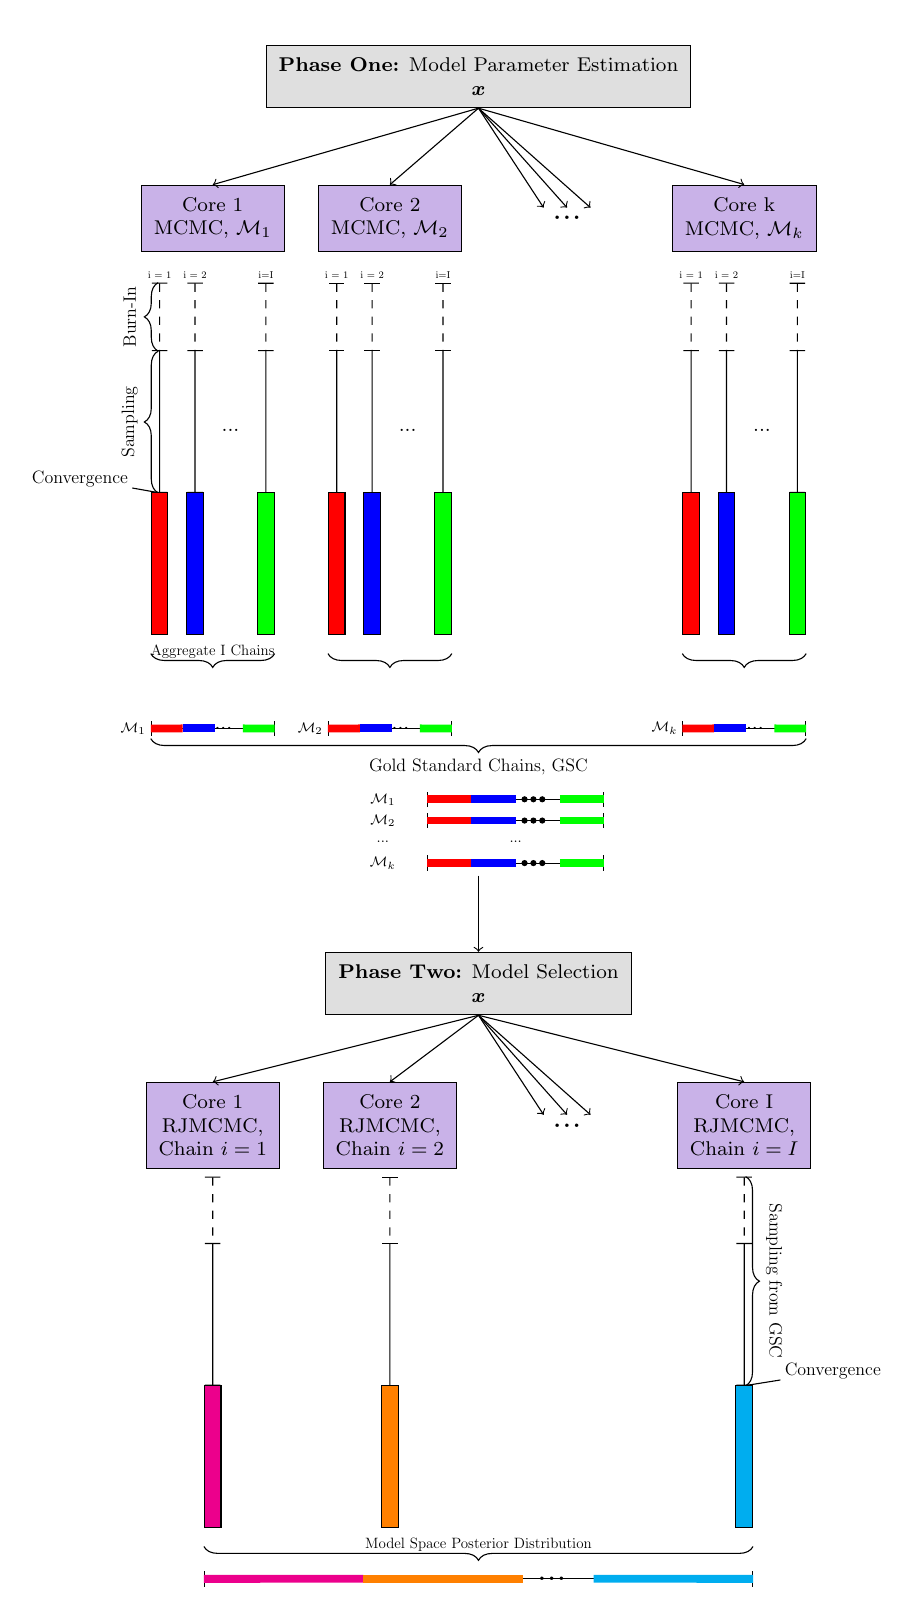
\begin{tikzpicture}[%
%every node/.style={transform shape},% now it's not necessary but good for a poster
scale = 0.9,
every node/.style = {transform shape},
x=1.25cm,y=2cm,  
font=\footnotesize,
% every group of nodes have a style except for main, the style is named by a letter
main/.style={draw,fill=lightgray!50,inner sep=.5em, align=center},
R/.style={draw,fill=purple!40!blue!30,inner sep=.5em, align=center},
M/.style={draw,fill=green!80!yellow,inner sep=.5em},
S/.style={anchor=east},
V/.style={anchor=west},
P/.style={anchor=center},
F/.style={anchor=west}
]

% main node Computer 
\node[main, label=above:] (computer) {\textbf{Phase One:} Model Parameter Estimation\\ $\data$};
%% wrappers
%\begin{scope}[on background layer]
%\node[fill=lightgray!50,inner sep = 4mm,fit=(computer)] {}; 
%\end{scope} 

%Draw Cores 
\node[R] at ($(computer)+(-3,-1)$)    (Core1+) {Core 1 \\MCMC, $\mathcal{M}_{1}$};
\node[R] at ($(computer)+(-1, -1)$)   (Core2+)  {Core 2 \\MCMC, $\mathcal{M}_{2}$};
\node[] at ($(computer)+(1, -1)$)   (CoreOther)  {\Large ...};
\node[R] at ($(computer)+(3,-1)$)   (Core3+) {Core k \\MCMC, $\mathcal{M}_{k}$};

%Draw lines 
\foreach \x in {1+, 2+,3+}{
	\draw[->] (computer.south) -- (Core\x.north);}

\draw[->] (computer.south) -- (CoreOther.north);
\draw[->] (computer.south) -- (CoreOther.north east);
\draw[->] (computer.south) -- (CoreOther.north west);

%Draw nodes for each chain
%Chain 1 
\foreach \x in {1+, 2+, 3+}{
	\node[align=center, scale=0.5] at ($(Core\x) +(-0.6,-0.4)$) (chain1Core\x) {i = 1};
	
	
	%Chain 2 	
	
	\node[align=center, scale=0.5] at ($(Core\x) +(-0.2,-0.4)$) (chain2Core\x) {i = 2};
	
	%Ellipses chain 
	
	\node[align=center] at ($(Core\x) +(0.2,-1.5)$) (chainExtraCore\x) {...};
	
	%Chain K 
	
	\node[align=center, scale=0.5] at ($(Core\x) +(0.6,-0.4)$) (chain3Core\x) {i=I};}

%%%%%%% Core 
%\node[align=center, scale=0.5] at ($(Core2+) +(-0.6,-0.4)$) (chain1Core2+) {i = 1};
%\node[align=center,scale = 0.5] at ($(Core2+) +(-0.2,-0.4)$) (chain2Core2+) {i = 2};
%\node[align=center, scale = 0.5] at ($(Core2+) +(0.2,-0.4)$) {...};
%\node[align=center, scale = 0.5] at ($(Core2+) +(0.6,-0.4)$) (chain3Core2+) {i = I};






%%%%%%%%%%%%%%Draw chain information %%%%%%%%%%%%%%%
%%% Burn In 
\foreach \core in {1+,2+, 3+}
\foreach \x in {1,2,3}{ 
	\node[] at ($(chain\x Core\core) + (0, -0.6)$) (burnChain\x Core\core) {};
	\draw [|-|, dashed] (chain\x Core\core) --(burnChain\x Core\core);}

%Label burn-in 
\draw[decorate,decoration={brace,amplitude=5pt,raise=0.5pt,mirror},yshift=0pt] (chain1Core1+.south) -- (burnChain1Core1+) node [midway,yshift=0pt, xshift =-12pt, rotate=90, scale=0.5]{\Large Burn-In};

%%% Samplign Path 
\foreach \core in {1+,2+, 3+}
\foreach \x in {1,2,3}{ 
	\node[] at ($(burnChain\x Core\core) + (0,-1)$) (sample\x Core\core) {};
	\draw [-|] (burnChain\x Core\core.north) -- (sample\x Core\core.north);}

%Label sample
\draw[decorate,decoration={brace,amplitude=5pt,raise=0.5pt,mirror},yshift=0pt] (burnChain1Core1+.north) -- (sample1Core1+) node [midway,yshift=0pt, xshift =-12pt, rotate=90, scale=0.5]{\Large Sampling};

%Annoteate Congernce 
\node[scale = 0.5] at ($(sample1Core1+.north) + (-0.9, 0.1)$) (convergeNode) {\Large Convergence}; 
\draw[-] (convergeNode) -- (sample1Core1+.north);


%Draw stead states 
\foreach \x in {1+, 2+, 3+}{
	%Make chain 1 red 
	\node[rectangle,draw,minimum width=0.1cm,minimum height=2cm, fill= red] at ($(sample1Core\x.north) + (0, -0.5)$) (ssp1Core\x) {};
	
	
	\node[] at ($(sample1Core\x) + (0,-1)$) (end1Core\x) {};
	
	%Make Chain 2 Blue 
	\node[rectangle,draw,minimum width=0.1cm,minimum height=2cm, fill= blue] at ($(sample2Core\x.north) + (0, -0.5)$) (ssp2Core\x) {};
	
	
	\node[] at ($(sample2Core\x) + (0,-1)$) (end2Core\x) {};
	
	%Make Chain 3 Green 
	\node[rectangle,draw,minimum width=0.1cm,minimum height=2cm, fill= green] at ($(sample3Core\x.north) + (0, -0.5)$) (ssp3Core\x) {};
	
	
	\node[] at ($(sample3Core\x) + (0,-1)$) (end3Core\x) {};}	

%Labe Steady state 
%\draw[decorate,decoration={brace,amplitude=5pt,raise=0.5pt,mirror},yshift=0pt] (ssp1Core1+.north) -- (end1Core1+) node [midway,yshift=0pt, xshift =-8pt, rotate=90, scale=0.5]{Steady State Path, $|SSP|$};

%Label Aggreation 
\draw[decorate,decoration={brace,amplitude=5pt,raise=0.5pt,mirror},yshift=0pt] (end1Core1+.south west) -- (end3Core1+.south east) node [midway,yshift=0pt, xshift =0pt, scale=0.5] (aggNode1+){\large Aggregate I Chains};

%Draw aggeration bracket for other chains 
\foreach \x in {2, 3}
\draw[decorate,decoration={brace,amplitude=5pt,raise=0.5pt,mirror},yshift=0pt] (end1Core\x +.south west) -- (end3Core\x+.south east) node [midway,yshift=0pt, xshift =0pt, scale=0.5] (aggNode\x +){};



%Draw an aggreatged chain 
%Add node lower than end core 
%Label model 
%
\foreach \x in {1,2,3}{
	\node[] at ($(end1Core\x +) + (0, -0.6)$) (aggStartCore\x +) {};
	\node[] at ($(end3Core\x +) + (0, -0.6)$) (aggEndCore\x +) {};
	
	%Draw node percent of teh way 
	\node[] at ($(aggStartCore\x +) !0.3! (aggEndCore\x +)$) (firstThirdCore\x +) {};
	\node[] at ($(aggStartCore\x +) !0.6! (aggEndCore\x +)$) (secondThirdCore\x +){};
	\node[] at ($(aggStartCore\x +) !0.6! (aggEndCore\x +)$)(thirdThirdCore\x +) {...};
	\node[] at ($(aggStartCore\x +) !0.7! (aggEndCore\x +)$)(finalThirdCore\x +) {};
	
	%Add thick lines to represent each sampling path. Try to make close to same length 
	\draw[|-|] (aggStartCore\x +.west) -- (aggEndCore\x +.east); 
	
	\draw[line width = 1mm, red] (aggStartCore\x +.west) -- (firstThirdCore\x +.west);
	\draw[line width = 1mm, blue] (firstThirdCore\x +.west) -- (secondThirdCore\x +.west);
	\draw[line width = 1mm, green] (finalThirdCore\x +.east) -- (aggEndCore\x +.east);}


%Labels nodes 
\foreach \x in {1,2}{
	\node[scale = 0.7] at ($(aggStartCore\x +.west) + (-0.2, 0)$) {$\mathcal{M}_{\x}$}; }

%Labeld Last model node node
\node[scale = 0.7] at ($(aggStartCore3+.west) + (-0.2, 0)$) {$\mathcal{M}_{k}$};

%Label and put all aggregtaed chains together 
\draw[decorate,decoration={brace,amplitude=5pt,raise=0.5pt,mirror},yshift=0pt] (aggStartCore1+.south west) -- (aggEndCore3+.south east) node [midway,yshift=-12pt, xshift =0pt, scale=0.5] {\Large Gold Standard Chains, GSC};

%Set nodes for chains 
\node[scale=0.7] at ($(aggStartCore1+) !0.35! (aggEndCore3+) + (0, -0.5)$) (model1Matrix) {$\mathcal{M}_{1}$};
\node[scale=0.7] at ($(model1Matrix) + (0, -0.15)$) (model2Matrix) {$\mathcal{M}_{2}$};
\node[scale=0.7] at ($(model2Matrix) + (0, -0.15)$) (blank1Matrix) {...};
\node[scale=0.7] at ($(blank1Matrix) + (1.5, 0)$) (blank2Matrix) {...};
\node[scale=0.7] at ($(blank1Matrix) + (0, -0.15)$) (model3Matrix) {$\mathcal{M}_{k}$};

%Add picture of aggreated chains for each model 
\foreach \x in {1,2,3}{
	\pic[scale =2] at ($(model\x Matrix) + (0.5, 0)$) {aggChain};}


%%%%%%%%%%%%%%%%%%%%%%%%%%%%%%%%%%%%%%%%%%%%%%%%%%%%%
%Start RJMCMC 
\node[] at ($(computer) + (0, -5.7)$) (blankNode) {}; 
\node[main, label=above:] at ($(computer) + (0,-6.4)$) (RJMCMC) {\textbf{Phase Two:} Model Selection\\ $\data$};

\draw[->] (blankNode.north) -- (RJMCMC);
% Draw cores for chain 
%Draw Cores 
\node[R] at ($(RJMCMC)+(-3,-1)$)    (RCore1+) {Core 1 \\RJMCMC, \\ Chain $i = 1$};
\node[R] at ($(RJMCMC)+(-1, -1)$)   (RCore2+)  {Core 2 \\RJMCMC, \\ Chain $i = 2$};
\node[] at ($(RJMCMC)+(1, -1)$)   (RCoreOther)  {\Large ...};
\node[R] at ($(RJMCMC)+(3,-1)$)   (RCore3+) {Core I \\RJMCMC, \\ Chain $i = I$};

%Draw lines 
\foreach \x in {1+, 2+,3+}{
	\draw[->] (RJMCMC.south) -- (RCore\x.north);}

\draw[->] (RJMCMC.south) -- (RCoreOther.north);
\draw[->] (RJMCMC.south) -- (RCoreOther.north east);
\draw[->] (RJMCMC.south) -- (RCoreOther.north west);


%Draw Line to represetn burn in and smapling 
%Draw nodes for each chain
%Chain 1 
\foreach \x in {1+, 2+, 3+}{
	\node[align=center] at ($(RCore\x) +(0,-0.3)$) (RchainCore\x) {};
	
	%Burn in 
	\node[] at ($(RchainCore\x) + (0, -0.6)$) (RburnChainCore\x) {};
	\draw [|-|, dashed] (RchainCore\x) --(RburnChainCore\x);
	
	%Sampling 
	\node[] at ($(RburnChainCore\x) + (0,-1)$) (RsampleCore\x) {};
	\draw [-|] (RburnChainCore\x.north) -- (RsampleCore\x.north);}


%Label sample Noting that we are samplign from SMM 
\draw[decorate,decoration={brace,amplitude=5pt,raise=0.5pt},yshift=0pt] (RchainCore3+.south) -- (RsampleCore3+) node [midway,yshift=0pt, xshift =12pt, rotate=270, scale=0.5]{\Large Sampling from GSC};

%Annoteate Congernce 
\node[scale = 0.5] at ($(RsampleCore3+.north) + (1, 0.1)$) (RconvergeNode) {\Large Convergence}; 
\draw[-] (RconvergeNode) -- (RsampleCore3+.north);


%Make chain 1 red 
\node[rectangle,draw,minimum width=0.1cm,minimum height=2cm, fill= magenta] at ($(RsampleCore1+.north) + (0, -0.5)$) (Rssp1Core1+) {};
\node[] at ($(RsampleCore1+) + (0,-1)$) (Rend1Core1+) {};


%Chain 2
\node[rectangle,draw,minimum width=0.1cm,minimum height=2cm, fill= orange] at ($(RsampleCore2+.north) + (0, -0.5)$) (Rssp1Core2+) {};
\node[] at ($(RsampleCore2+) + (0,-1)$) (Rend1Core2+) {};

%Chain 3
\node[rectangle,draw,minimum width=0.1cm,minimum height=2cm, fill= cyan] at ($(RsampleCore3+.north) + (0, -0.5)$) (Rssp1Core3+) {};	
\node[] at ($(RsampleCore3+) + (0,-1)$) (Rend1Core3+) {};


%Label Aggreation 
\draw[decorate,decoration={brace,amplitude=5pt,raise=0.5pt,mirror},yshift=0pt] (Rend1Core1+.south west) -- (Rend1Core3+.south east) node [midway,yshift=0pt, xshift =0pt, scale=0.5] (RaggNode1+){\large Model Space Posterior Distribution};



\node[] at ($(Rend1Core1+) + (0, -0.3)$) (RaggStartCore1+) {};
\node[] at ($(Rend1Core3+) + (0, -0.3)$) (RaggEndCore1+) {};

%Draw node percent of teh way 
\node[] at ($(RaggStartCore1+) !0.3! (RaggEndCore1+)$) (RfirstThirdCore1+) {};
\node[] at ($(RaggStartCore1+) !0.6! (RaggEndCore1+)$) (RsecondThirdCore1+){};
\node[] at ($(RaggStartCore1+) !0.6! (RaggEndCore1+)$)(RthirdThirdCore1+) {\Large \hspace{0.4cm} ...};
\node[] at ($(RaggStartCore1+) !0.7! (RaggEndCore1+)$)(RfinalThirdCore1+) {};

%Add thick lines to represent each sampling path. Try to make close to same length 
\draw[|-|] (RaggStartCore1+.west) -- (RaggEndCore1+.east); 

\draw[line width = 1mm, magenta] (RaggStartCore1+.west) -- (RfirstThirdCore1+.west);
\draw[line width = 1mm, orange] (RfirstThirdCore1+.west) -- (RsecondThirdCore1+.west);
\draw[line width = 1mm, cyan] (RfinalThirdCore1+.east) -- (RaggEndCore1+.east);
%A test
\end{tikzpicture} 

\end{document}  